%!TEX root = ../../tcc.tex

\section{IPv6}

Com o desenvolvimento da ARPAnet, a quantidade de computadores conectados na rede
cresceu, chegando a 562 em 1983. A quarta versão do protocolo TCP/IP, o IPv4, foi
criado em 1981 \cite{site:rfcipv4}, foi utilizado para organizar aquelas redes já
formadas e ordenar o crescimento posterior.

O IPv4 tem dois objetivos: prover a fragmentação dos datagramas maiores em partes
menores, para que pudessem ser enviados pela camada de enlace; e regras de
endereçamento, para que os datagramas tivessem os endereços de origem e de destino
armazenados em seus cabeçalhos \cite{site:nicipv4}. Apesar de ser considerada robusta e
de fácil implantação e interoperabilidade, o projeto original não previu problemas como
o crescimento das redes e das tabelas de roteamento, segurança de dados, prioridade de
entrega de tipos específicos de pacote e, o mais grave, o esgotamento de endereços IP.

O endereçamento do IPv4 é feito com 4 bytes, geralmente representado na forma decimal
(4 números de 0 a 255), separados por pontos, o que permite $2^32$ endereços possíveis.
Esses endereços, que são distribuídos pela IANA
(\emph{Internet Assigned Numbers Authority}) globalmente para os cinco RIRs
(\emph{Regional Internet Registry}, ou Registro Regional de Internet), que então
distribuem localmente para clientes que incluem provedores de Internet (\glspl{isp}) e
outras organizações, que então repassam endereços a usuários finais. Esses endereços
são os que estão esgotando atualmente. Para resolver esse problema e alguns outros que
adquiridos com a experiência operacional do IPv4, o IPv6 foi publicado em 1998
\cite{site:rfcipv6}.

O IPv6 possui várias alterações desde o IPv4, muitas delas evidentes no formato do seu
datagrama:

\begin{description}
    \item[espaço de endereço maior:] o tamanho dos endereços passa a ter 128 bits,
        representados em 8 grupos de 4 dígitos hexadecimais. Com isso, a quantidade
        total de endereços possíveis passa de $2^32$ para $2^128$. Isso também permitiu
        que fossem definidas três metodologias de roteamento: o \emph{unicast} (para um
        endereço em específico), o \emph{multicast} (para vários endereços
        simultaneamente) e o \emph{anycast} (para, dentre um grupo de potenciais
        destinatários, apenas um receba);

    \item[cabeçalho de 40 bytes fixos:] o cabeçalho do IPv4 possui alguns campos
        opcionais, porém alguns deles foram retirados ou sofreram alterações quando
        migrados para o IPv6. Isso agiliza o processamento dos datagramas; e

    \item[classificação de fluxo e prioridade:] permite que dados que sejam de fluxo
        contínuo, como áudio ou vídeo, possam ter tratamento diferenciado no
        redirecionamento de pacotes e melhor manipulação da qualidade para serviços
        específicos.
\end{description}

\begin{figure}[H]
    \centering
    \fbox{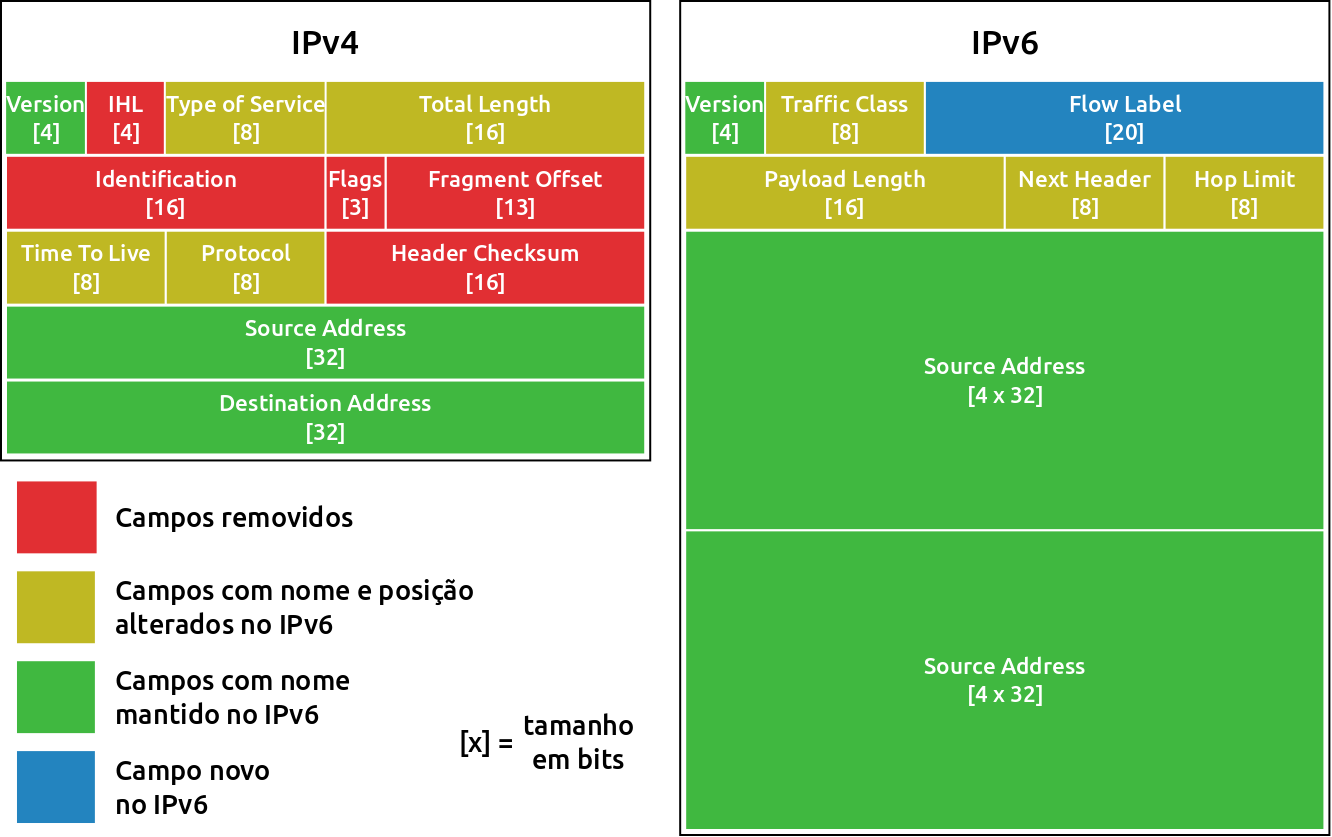
\includegraphics[width=\textwidth]{IPheaders.png}}
    \caption{formatos dos datagramas dos protocolos IPv4 e IPv6. Ambos possuem largura de 32 bits}
    \label{fig:headers}
\end{figure}

Os campos do cabeçalho do IPv6 são:

\begin{description}
    \item[Version:] traz a versão do protocolo utilizado (no caso do IPv6, o valor 6).
        Porém, o simples envio do valor 4 não implica na utilização do IPv4, não
        possuindo compatibilidade anterior;

    \item[Traffic Class:] campo de 8 bits que possui a mesma finalidade do campo
        \emph{Type of Service} no IPv4, que especifica que o datagrama possui dados que
        requerem tráfego com baixo atraso, alta vazão ou confiabilidade;

    \item[Flow Label:] campo de 20 bits usado na classificação de fluxo de datagramas;

    \item[Payload Length:] campo de 16 bits que representa um inteiro positivo para o
        tamanho do conjunto de dados anexado após o cabeçalho;

    \item[Next Header:] identifica o protocolo usado para entregar os dados (\gls{tcp}
        ou \gls*{udp}). É usado da mesma forma que no IPv4;

    \item[Hop Limit:] quantidade máxima de roteadores pelos quais o datagrama poderá
        passar, sendo decrescido de 1 cada vez que passa por algum. Quando chega a 0, o
        datagrama é descartado; e

    \item[Source Address e Destination Address:] endereços IPv6 de origem e de destino
        do datagrama, em alguma das várias representações possíveis definidas no RFC4291
        \cite{site:rfcipv6add}.
\end{description}

Duas ausências significativas foram as dos campos que definem a fragmentação dos
datagramas e do \gls{checksum} do cabeçalho. No primeiro, a funcionalidade foi movida
dos roteadores, a fim de reduzir o trabalho deles e melhorar a velocidade do
encaminhamento IP pela rede, e tornando os sistemas finais responsáveis pela escolha do
tamanho dos datagramas. Já o \gls*{checksum}, os protocolos das camadas de transporte
(\gls*{tcp} e \gls*{udp}) e de enlace (Ethernet) já realizam a verificação de erros por
soma. Por isso, a redundância de trabalho foi retirada, eliminando a necessidade de
recalcular essa soma a cada roteador e, assim, melhorar a velocidade de processamento de
pacotes IP.

Apesar de não ser retrocompatível com o IPv4, o IPv6 consegue ser transmitido utilizando
\textbf{tunelamento automático} por \textbf{mecanismos de transição}, que proporciona
uma camada transparente para que pacotes IPv6 transitem em uma rede IPv4. Entre esses
mecanismos estão o 6to4, 6in4 e Teredo.

%!TEX root = ../../tcc.tex

\subsection*{Uso do IPv6}

O IPv6 tem duas datas marcantes: o Dia Mundial e o Dia do Lançamento Mundial do IPv6.
No Dia Mundial do IPv6, ou \emph{World IPv6 Day}, organizado pelo
\emph{Internet Society} (ISOC) \cite{site:isoc-ipv6day}, ocorreu no dia 8 de junho de
2011 UTC e contou com a participação de grandes empresas estrangeiras (Facebook,
Google, Yahoo!, Akamai, Lamelight Networks, etc) e brasileiras (Terra, Campus Party,
IG), num teste de 24 horas de oferecimento de conexão e conteúdo utilizando o protocolo
IPv6. O evento foi considerado um sucesso pela ISOC.

Já o Dia de Lançamento Mundial do IPv6, no dia 6 de junho de 2012, foi um evento
semelhante ao Dia Mundial, com o mesmo objetivo e com mais participantes, porém mantendo
o IPv6 habilitado após o evento \cite{site:isoc-ipv6launch}. Desde então, empresas do
mundo todo têm corrido contra o relógio para que o oferecimento de conexões de Internet
não seja estagnado pela falta de endereços.

O IPv6 precisa ser suportado pelas pontas das redes (aplicações em clientes e
servidores) e pelas rotas entre eles (provedores de acesso, empresas de
telecomunicações). Enquanto o primeiro é simples, pois bastam configurações de
conectores dos respectivos sistemas operacionais, servidores de aplicação e roteadores
internos que suportem o IPv6, o caminhos entre ambos é mais complicado. Para as empresas
provedoras de acesso, envolvem custos de troca de equipamentos da infraestrutura de
rede, além do treinamento da mão de obra. Por conta disso, a transição para o novo
protocolo ainda é complexa e lenta.

O contexto brasileiro do IPv6 a situação está devagar. Segundo o SindiTelebrasil em
novembro de 2013 \cite{site:ipv6brasil}, as operadoras brasileiras ainda estavam
adquirindo equipamentos. O cenário era considerado preocupante, e devido ao atraso da
migração tecnológica, medidas paliativas estão sendo tomadas.

Uma delas é o compartilhamento de endereços IPv4 por usuários, com restrição de portas,
que pode afetar a experiência de uso de alguns tipos de aplicações. Esse
compartilhamento é feito usando-se dois \glspl*{nat}, usando o modelo de \gls*{nat}444.

\begin{figure}[H]
    \centering
    \fbox{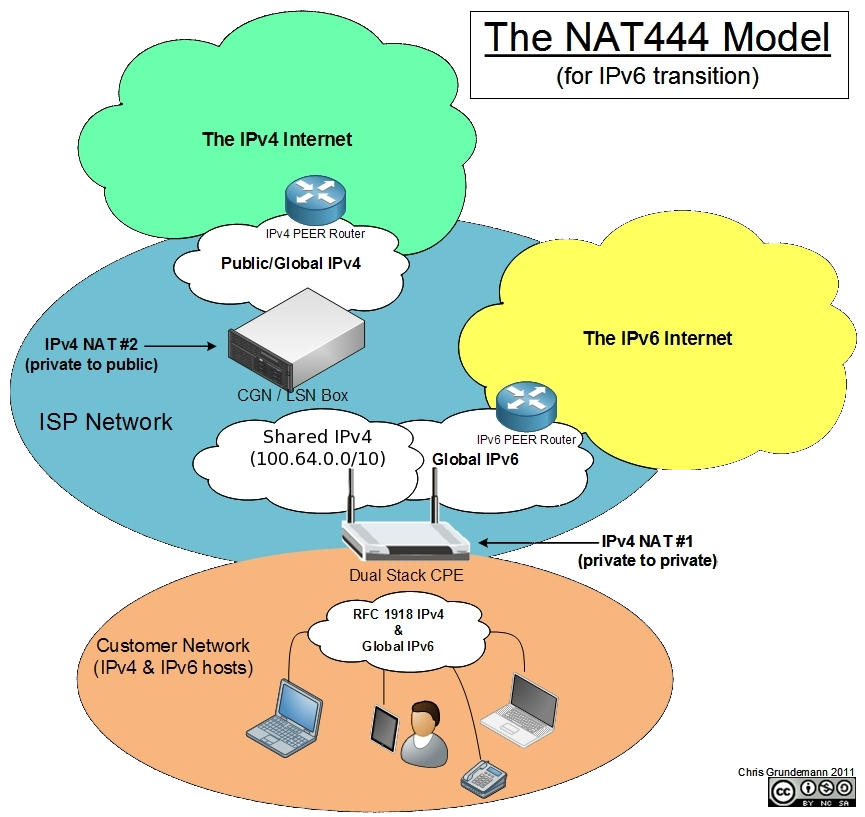
\includegraphics[width=\textwidth]{nat444.png}}
    \caption{Esquema de uso do NAT444. Fonte:\cite{site:nat444}}
    \label{fig:nat444}
\end{figure}

No \gls*{nat}444 \cite{site:nat444}, dois \glspl*{nat} são usados, e é possível perceber que:

\begin{itemize}
    \item \gls*{nat}444 de IPv4 funcionando em pilha dupla (\emph{dual stacked}; para
        ambos os protocolos) com IPv6 global (público); e

    \item \gls*{nat}444 adiciona uma segunda camada de \gls*{nat}, ou seja, uma segunda
        área de endereçamento ``interno'' (privada).
\end{itemize}

Ao adicionar a segunda camada, vários usuários podem ter um mesmo endereço, ou seja, o
\gls*{isp} deverá tomar medidas como registrar os acessos com as respectivas portas de
entrada e saída, por questões legais. Outro fato é que deve-se aceitar que o segundo
\gls*{nat} não será configurável por UPnP, por \gls*{nat}-PMP ou outros protocolos de
travessia de \gls*{nat}. Um \gls*{isp} não permitirá que ocorra essa configuração, pois
existirá o risco de um usuário afetar serviços de outros. Por esse motivo, pode-se
prever aplicações que podem ser afetadas com problemas de desempenho ou mesmo
incapacidade de execução \cite{site:rfcnat444}:

\begin{itemize}
    \item grandes downloads por FTP
    \item \emph{seeding} em Limewire e BitTorrent
    \item jogos online (Xbox, Playstation, etc)
    \item \emph{streaming} de vídeo (Hulu, Netflix, etc)
    \item acesso remoto de webcam
    \item tunelamento para IPv6 (6to4, Teredo, etc)
    \item VPN e criptografia (IPSec, SSL)
    \item VoIP
\end{itemize}